% ============================================
% DEFINICIÓN DE FUENTE PARA LA PORTADA
% ============================================
\newfontfamily\montserrat[
  Path=assets/fuentes/Montserrat/static/,
  Extension=.ttf,
  BoldFont=Montserrat-SemiBold,
  ItalicFont=Montserrat-Italic  % Si no existe, fontspec usará slant sintético
]{Montserrat-Regular}

%=============================================================================
% PÁGINA 2: PORTADA FULL-PAGE
%=============================================================================
{

\thispagestyle{empty}

\hoffset=-1in
\voffset=-1in
\oddsidemargin=0pt
\evensidemargin=0pt
\topmargin=0pt
\headheight=0pt
\headsep=0pt

\noindent
% El comando \lower agarra la caja de ancho cero y la desplaza hacia abajo de forma obligatoria.
% Empezamos con 1.8cm. Si notas que le falta bajar un poco, súbelo a 2.5cm.
\lower 1.8cm \hbox to \paperwidth{%
    \hss
    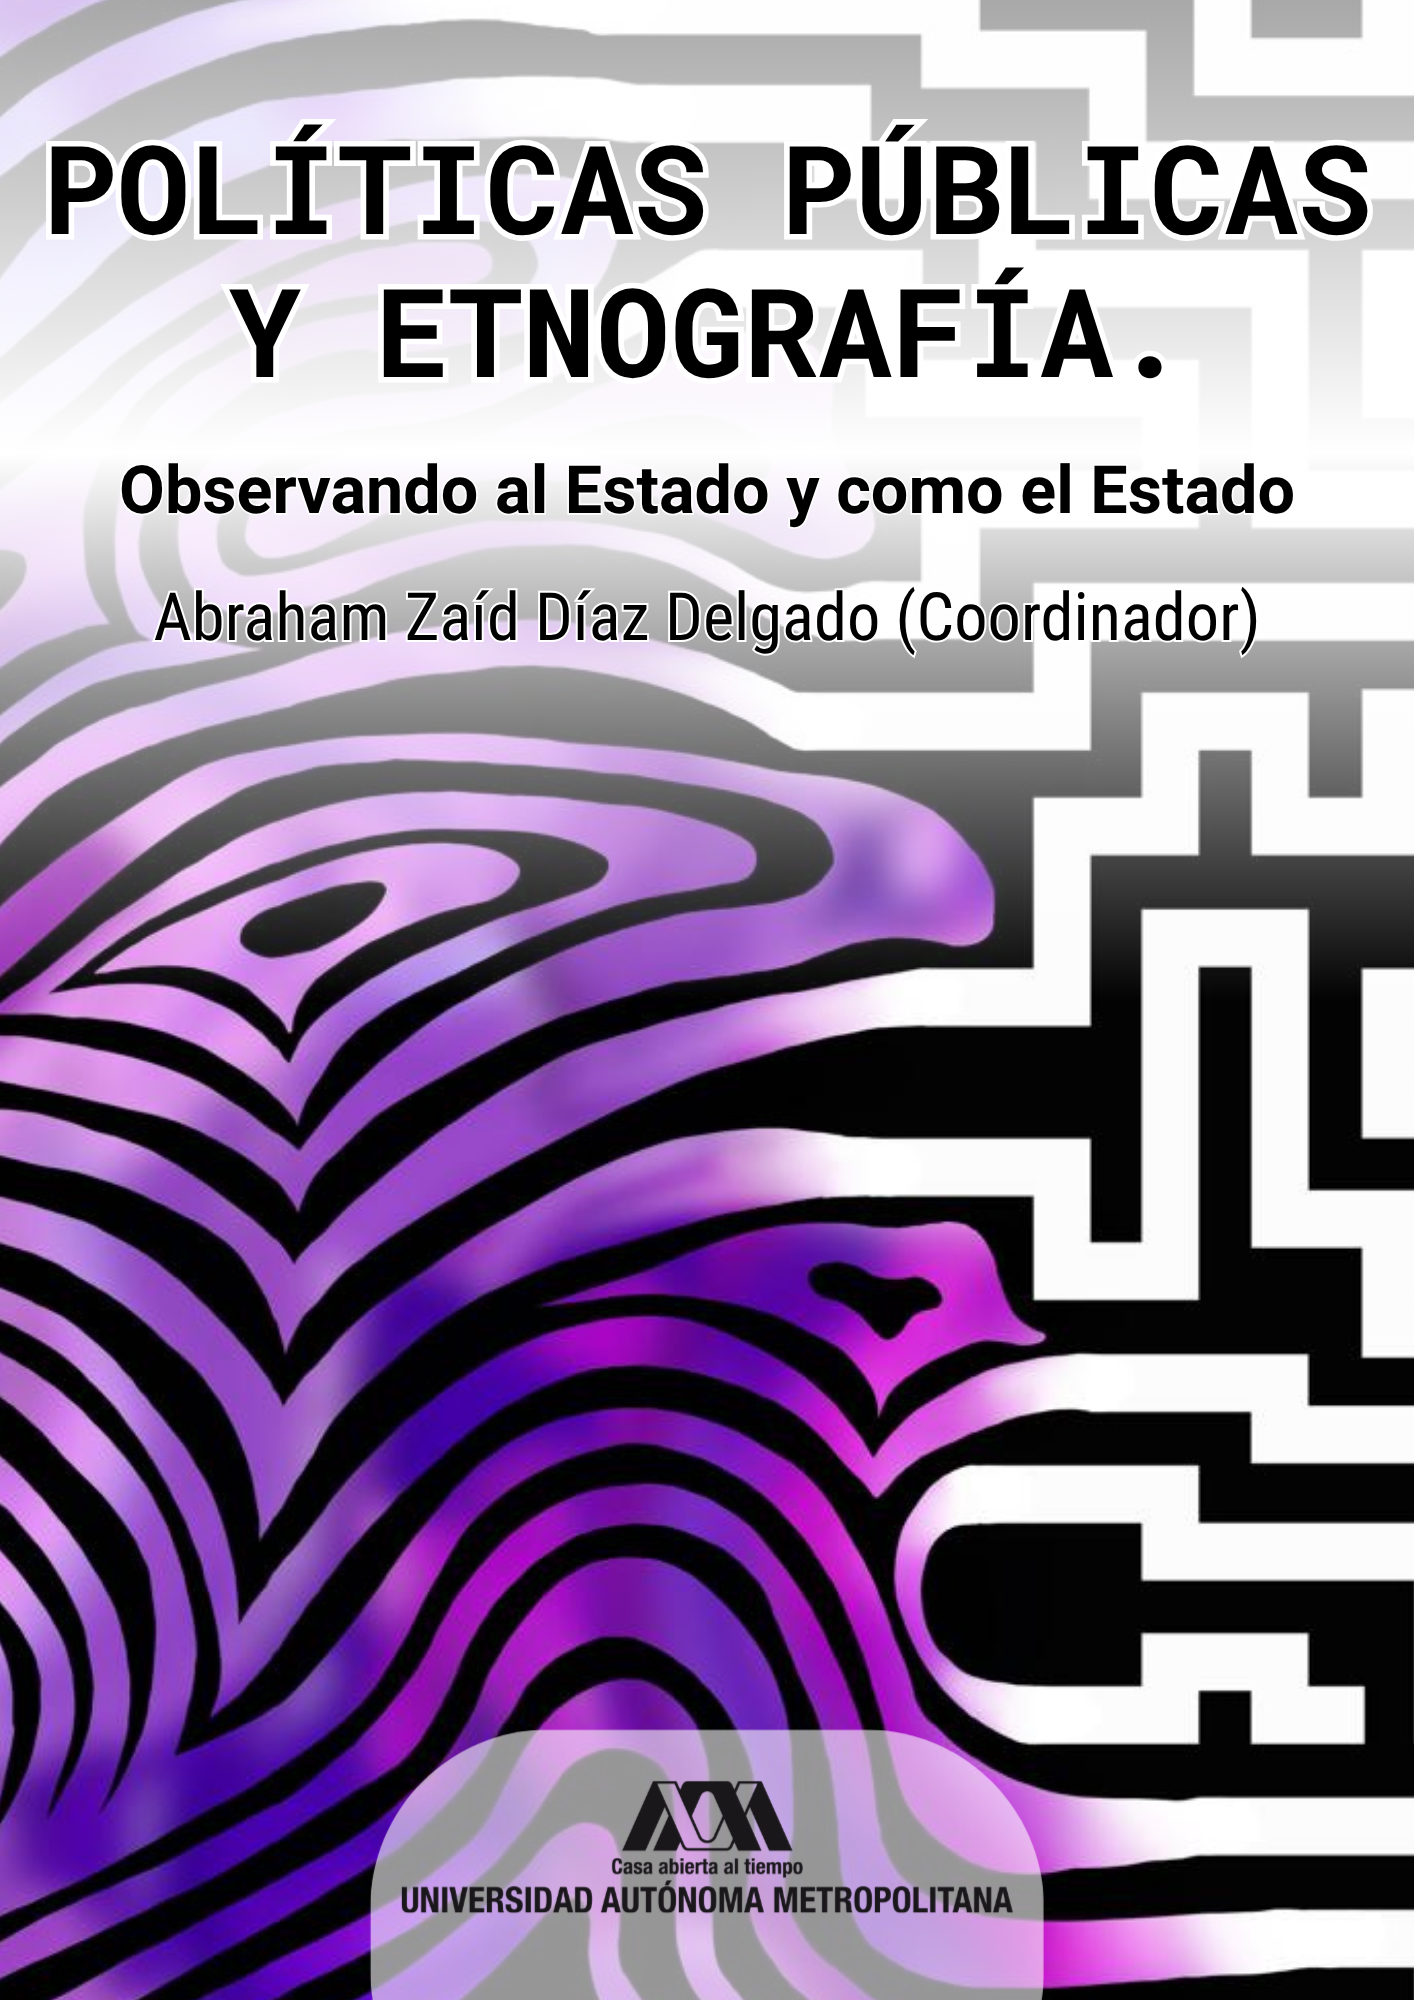
\includegraphics[width=\paperwidth,height=1.0\paperheight,keepaspectratio=false]{assets/imagenes/libro2_portada_2026.png}%
    \hss
}

\clearpage

}
% ============================================
% PÁGINA 2: EN BLANCO (verso de portada)
% ============================================
\clearpage
\thispagestyle{empty}
\null
\clearpage

% ============================================
% PÁGINA 3: PORTADILLA (MEDIA PORTADA)
% ============================================
\clearpage
  \thispagestyle{empty}
  \begingroup
    \raggedright
    \vspace*{1cm}
    \sffamily\small
    \montserrat\huge Políticas Públicas y Etnografía \\
    \vspace{0.3cm}
    {\Large Observando al Estado y como el Estado} \\
    \vspace{0.7cm}
    {\Large Abraham Zaíd Díaz Delgado} \\
    \vspace{0.3cm}
    \Large\rmfamily\textit{Coordinador}
    \vfill
    \begin{minipage}[t]{0.50\textwidth}
        
\includegraphics[width=1.2\textwidth]{../../assets/logos/logo_uam_l.png}
    \end{minipage}
  \endgroup
\clearpage

% ==============================================================================
% PÁGINA 4: DIRECTORIO INSTITUCIONAL CENTRADO (Solo Unidad Lerma)
% ==============================================================================
\clearpage
  \begingroup
    \thispagestyle{empty}
      \begin{center}
        \sffamily\small
        {\montserrat\Large\textbf{UNIVERSIDAD AUTÓNOMA METROPOLITANA}} \\
        {\montserrat\large\textbf{UNIDAD LERMA}} \\
        \vspace{0.4cm}
        \textit{Dra. Alma Patricia de León Calderón} \\
        Rectora \\
        \vspace{0.3cm}
        \textit{Mtra. Luz del Carmen Alitzel Almaraz Calderón} \\
        Secretaria \\
        \vspace{0.3cm}
        \textit{Dr. Raúl Hernández Mar} \\
        Director de la División de Ciencias Sociales y Humanidades \\
        \vspace{0.3cm}
        \textit{Dra. Ana Carolina Robles Salvador} \\
        Secretaria Académica de la División de Ciencias Sociales y Humanidades \\
  
        \vspace{0.5cm}
        \rule{0.6\textwidth}{0.4pt}
        \vspace{0.5cm}
  
        {\montserrat\large\textbf{COMITÉ EDITORIAL}} \\
        {\montserrat\large\textbf{DIVISIÓN DE CIENCIAS SOCIALES Y HUMANIDADES}} \\
        {\montserrat\normalfont{PUBLICACIONES PERIÓDICAS}} \\
        \vspace{0.4cm}
        \textit{Abigail Martínez Mendoza} \\
        Coordinadora General \\
        \vspace{0.3cm}
        \textit{Omar Valencia Domínguez} \\
        \textit{Ryszard Edward Rozga Luter} \\
        Departamento de Procesos Sociales \\
        \vspace{0.3cm}
        \textit{José Omar Pérez Baños} \\
        Departamento de Estudios Culturales \\
        
        \vspace{0.5cm}
        \rule{0.6\textwidth}{0.4pt}
        \vspace{0.5cm}
        
        {\montserrat\large\textbf{EDICIÓN TÉCNICA, CORRECCIÓN DE ESTILO y DISEÑO}} \\
        \vspace{0.4cm}
        \textit{José Omar Pérez Baños}\\
        \textit{Jonathan Armando Chávez Solís}\\
        \textit{Yunuen Rosas Ortíz}\\
      \end{center}
  \endgroup
\clearpage

% ==============================================================================
% PÁGINA 5: PÁGINA LEGAL ESTÁNDAR (DCSH - UAM LERMA)
% ==============================================================================
\clearpage
\thispagestyle{empty}
\begin{center}
    % --- Ficha de Catalogación Superior ---
    \framebox[\textwidth]{\vbox{
        \vspace{0.3cm}
        \hbox to \textwidth{\hfill\montserrat\scriptsize\textbf DATOS DE CATALOGACIÓN\hfill}
        \vspace{0.2cm}
        \noindent\hspace{0.5cm}
        \parbox{0.9\textwidth}{
            \rmfamily\scriptsize
            \texttt{Díaz Delgado, Abraham Zaíd (coordinador)} \\
            Políticas Públicas y Etnografía : Observando al Estado y como el Estado / Abraham Zaíd Díaz Delgado, coordinador. -- México : Universidad Autónoma Metropolitana : Unidad Lerma : División de Ciencias Sociales y Humanidades, 2026. \\
            \quad p. : il. ; 14 x 21 cm. \\
            \quad ISBN: 978-xxx-xxx-xxx-x \\
            \quad 1. Políticas públicas -- Aspectos sociales. 2. Etnografía -- Metodología -- México. I. Universidad Autónoma Metropolitana. Unidad Lerma. División de Ciencias Sociales y Humanidades.
        }
        \vspace{0.3cm}
    }}
\end{center}

\vspace*{\fill} % Empuja los datos legales al fondo de la página

% --- Créditos y Derechos de Autor ---

\begingroup
\begin{singlespace}
\fontspec{Montserrat-Regular.otf}\scriptsize
\noindent
Primera edición: 2026\\
Políticas Públicas y Etnografía : Observando al Estado y como el Estado\\
Abraham Zaíd Díaz Delgado, coordinador\\[0.5em]
Diseño de portada: Yunuen Rosas Ortíz\\[0.5em]
D.R. © 2026, Universidad Autónoma Metropolitana\\
Prolongación Canal de Miramontes 3855, Ex Hacienda San Juan de Dios,\\
Alcaldía de Tlalpan, C.P. 14387, Ciudad de México.\\[0.5em]
{\fontspec{Montserrat-SemiBold.otf}\scriptsize Universidad Autónoma Metropolitana, Unidad Lerma}\\
División de Ciencias Sociales y Humanidades\\
Consejo Editorial de la División de Ciencias Sociales y Humanidades\\
Avenida de las Garzas núm. 10, Col. El Panteón,\\
C.P. 52005, Lerma de Villada, Estado de México.\\
\texttt{<correo.editorial@correo.lerma.uam.mx>}\\[0.8em]
ISBN: 978-xxx-xxx-xxx-x\\[0.8em]
Esta publicación no puede ser reproducida, ni en todo ni en parte, ni registrada o transmitida por un sistema de recuperación de información, en ninguna forma ni por ningún medio, sea mecánico, fotoquímico, electrónico, magnético, electroóptico, por fotocopia o cualquier otro, sin el permiso previo y por escrito de los editores.\\[0.5em]
La presente publicación pasó por un proceso de dos dictámenes (doble ciego) de pares académicos avalados por el Consejo Editorial de la División de Ciencias Sociales y Humanidades de la UAM-Lerma, que garantizan su calidad y pertinencia académica y científica.\\[0.5em]
Impreso en México / Printed in Mexico
\end{singlespace}
\endgroup
\clearpage

% ============================================
% PÁGINA EN BLANCO
% ============================================
\clearpage
\thispagestyle{empty}
\null
\clearpage